% Options for packages loaded elsewhere
\PassOptionsToPackage{unicode}{hyperref}
\PassOptionsToPackage{hyphens}{url}
%
\documentclass[
]{article}
\usepackage{amsmath,amssymb}
\usepackage{lmodern}
\usepackage{iftex}
\ifPDFTeX
  \usepackage[T1]{fontenc}
  \usepackage[utf8]{inputenc}
  \usepackage{textcomp} % provide euro and other symbols
\else % if luatex or xetex
  \usepackage{unicode-math}
  \defaultfontfeatures{Scale=MatchLowercase}
  \defaultfontfeatures[\rmfamily]{Ligatures=TeX,Scale=1}
\fi
% Use upquote if available, for straight quotes in verbatim environments
\IfFileExists{upquote.sty}{\usepackage{upquote}}{}
\IfFileExists{microtype.sty}{% use microtype if available
  \usepackage[]{microtype}
  \UseMicrotypeSet[protrusion]{basicmath} % disable protrusion for tt fonts
}{}
\makeatletter
\@ifundefined{KOMAClassName}{% if non-KOMA class
  \IfFileExists{parskip.sty}{%
    \usepackage{parskip}
  }{% else
    \setlength{\parindent}{0pt}
    \setlength{\parskip}{6pt plus 2pt minus 1pt}}
}{% if KOMA class
  \KOMAoptions{parskip=half}}
\makeatother
\usepackage{xcolor}
\usepackage{graphicx}
\makeatletter
\def\maxwidth{\ifdim\Gin@nat@width>\linewidth\linewidth\else\Gin@nat@width\fi}
\def\maxheight{\ifdim\Gin@nat@height>\textheight\textheight\else\Gin@nat@height\fi}
\makeatother
% Scale images if necessary, so that they will not overflow the page
% margins by default, and it is still possible to overwrite the defaults
% using explicit options in \includegraphics[width, height, ...]{}
\setkeys{Gin}{width=\maxwidth,height=\maxheight,keepaspectratio}
% Set default figure placement to htbp
\makeatletter
\def\fps@figure{htbp}
\makeatother
\setlength{\emergencystretch}{3em} % prevent overfull lines
\providecommand{\tightlist}{%
  \setlength{\itemsep}{0pt}\setlength{\parskip}{0pt}}
\setcounter{secnumdepth}{-\maxdimen} % remove section numbering
\ifLuaTeX
  \usepackage{selnolig}  % disable illegal ligatures
\fi
\IfFileExists{bookmark.sty}{\usepackage{bookmark}}{\usepackage{hyperref}}
\IfFileExists{xurl.sty}{\usepackage{xurl}}{} % add URL line breaks if available
\urlstyle{same} % disable monospaced font for URLs
\hypersetup{
  hidelinks,
  pdfcreator={LaTeX via pandoc}}

\author{}
\date{}

\begin{document}

Description: A breakdown of basic statistics and its notation.

\hypertarget{basic-statistics}{%
\section{Basic Statistics}\label{basic-statistics}}

\hypertarget{what-is-the-bernoulli-and-binomial-distribution}{%
\subsubsection{What is the bernoulli and binomial distribution
?}\label{what-is-the-bernoulli-and-binomial-distribution}}

Bernoulli distribution: The random variable can either be 0 or 1.
Binomial distribution: The random variable remains to have only two
states, this shows the probability of measuring either state x number of
times given n independent occurrences.

\hypertarget{what-is-the-mean-expectation-and-standard-deviation}{%
\subsubsection{What is the mean, expectation and standard
deviation?}\label{what-is-the-mean-expectation-and-standard-deviation}}

The mean is the frequency of each value occurring, multiplied by the
value all summed for each random variable.

\(\overline{x} = 1/n(\Sigma fx)\)

The expectation is the probability of each value multiplied by the
value, summed for all values. This is the value the mean tends to as the
sample size increases.

\(E(x) = \Sigma x P(X=x)\)

The variance is the average of the squared difference from the mean.

\(\sigma^2 = E(X^2) - (E(X))^2\)

The standard deviation is the square root of the variance, showing
essentially the average distance from the mean.

\(\sigma\)

An overall shift to all data points will effect expectation and not
variance:

\(E(X \pm a) = E(X) \pm a\)

\(Var(X \pm a) = Var(X)\)

An overall multiplier to all data points effects both expectation and
variance:

\(E(aX) = aE(X)\)

\(Var(aX) = a^2Var(X)\)

\hypertarget{poisson-distribution}{%
\subsection{Poisson Distribution}\label{poisson-distribution}}

\hypertarget{what-is-the-poisson-distribution}{%
\subsubsection{What is the poisson distribution
?}\label{what-is-the-poisson-distribution}}

\begin{itemize}
\tightlist
\item
  Random discrete variable is a count of the number of events occurring
  at random in regions of time and space.

  \begin{itemize}
  \tightlist
  \item
    All events are independent
  \item
    No two events at the same time
  \item
    Over a short period of time or on a small region the probability is
    the same
  \end{itemize}
\end{itemize}

\(p_x = P(X=x) = e^-\lambda *\lambda^x/x!\)

Recurrence formula:

\(P(X=x) = \lambda/x * P(X= x-1)\)

\(\lambda\) is the mean var and \(\sqrt(\lambda)\) is the std

95\% of values are between the mean \(\pm\) 2 std

Independent Poisson random variables can be added to give another
Poisson random variable

\hypertarget{continuos-variables}{%
\subsection{Continuos variables}\label{continuos-variables}}

\hypertarget{what-is-the-difference-between-continuos-and-discrete-variables}{%
\subsubsection{What is the difference between continuos and discrete
variables
?}\label{what-is-the-difference-between-continuos-and-discrete-variables}}

Discrete variables are a known list of possible numbers

Continuos random variables are infinite.

\hypertarget{what-is-relative-frequency-density-and-how-does-it-translate-to-probability}{%
\subsubsection{What is relative frequency density and how does it
translate to
probability?}\label{what-is-relative-frequency-density-and-how-does-it-translate-to-probability}}

The relative frequency density; is a measurement of the relative
frequency over a class width (interval between two values)

\(\frac{Relative frequency}{class width} = Relative frequency density\)

The probability density function f(x); is the relative frequency density
as n increases and the class width decreases

Area under a plotted f(x) gives the probability for that range of
continuos variables.

\(P(X<x) = \int_{-\infin}^{x} f(x)\)

\(\frac{d}{dx}P(X<x) = f(x)\)

You cannot get the probability for a specific value via f(x):

\(P(X=k) = 0\)

\hypertarget{how-do-you-calculate-the-median}{%
\subsubsection{How do you calculate the
Median?}\label{how-do-you-calculate-the-median}}

The median value (m) is when the probability for values above and below
are 0.5.

\(\int_{m}^{\inf} f(x) = 0.5\)

\hypertarget{how-do-you-calculate-a-percentile}{%
\subsubsection{How do you calculate a
Percentile?}\label{how-do-you-calculate-a-percentile}}

The Xth percentile is the value below which the probability is X/100:

90th percentile

\(P(X<x_{90th}) = 0.9\)

\hypertarget{how-do-you-calculate-the-mean}{%
\subsubsection{How do you calculate the
Mean?}\label{how-do-you-calculate-the-mean}}

If assume the a small width of delta x, the mean will be
\(\sum x(f(x)\delta(x))\) (the brackets give the probabilty and
multiplying by x gives the mean). As delta x tends to 0 this becomes:

\(\bar{x} = \int xf(x)\)

The population mean is then :

\(\mu = \int_{-\infty}^{\infty} xf(x) dx\)

The variance is:

\(Var(x) = \int_{-\infty}^{\infty} (x -\mu)^2 f(x) dx\)

\hypertarget{estimation}{%
\subsection{Estimation}\label{estimation}}

\hypertarget{confidence-interval}{%
\subsubsection{Confidence Interval}\label{confidence-interval}}

\hypertarget{what-is-a-normal-distribution}{%
\subsubsection{what is a normal distribution
?}\label{what-is-a-normal-distribution}}

\textbf{Normal distribution} : Data set centered evenly about a value,
giving a bell curve.

\hypertarget{how-do-you-calculate-the-confidence-interval}{%
\subsubsection{How do you calculate the confidence interval
?}\label{how-do-you-calculate-the-confidence-interval}}

To calculate the confidence interval of a population mean, use the
variable Z below, where \(\bar{X}\) is variable corresponding to the
sample mean:

\(Z = (\bar{X} - \mu)/ (\sigma/ \sqrt{n}\))

For a normal distribution with mean 0 and std of 1 N(0,1) the confidence
interval is:

\((\bar{x} - 1.96 (\sigma/\sqrt{n}),\bar{x} - 1.96 (\sigma/\sqrt{n}))\)

The above interval on an average of 95\% of the time will include the
mean.

\hypertarget{what-is-a-t-distribution}{%
\subsubsection{What is a T
Distribution?}\label{what-is-a-t-distribution}}

If the the sample size is limited and below 30, then instead of a normal
and T distribution is used.

A T dist has degrees of freedom (v) = n-1:

\begin{itemize}
\tightlist
\item
  A normal distribtion has degrees of freedom v = \(\infty\)
\item
  n being the sample size
\end{itemize}

If the variance is unknown and n is large, Z can be adjusted to use
s\^{}2 which is an unbiased estimate of the variance. This gives two
random variables in the equation X and S:

\(T = (\bar{X} - \mu)/ (S/\sqrt{n})\)

c is the critical value depending on the distribution parameters and the
confidence interval required:

\((\bar{x} + c(s\sqrt{n}),\bar{x} - c(s\sqrt{n}))\)

\hypertarget{how-is-s-calculated}{%
\subsubsection{How is s calculated ?}\label{how-is-s-calculated}}

\(s^2 = 1/(n-1) * \sum(x-\bar{x})^2\)

\hypertarget{hypothesis-testing}{%
\subsection{Hypothesis testing}\label{hypothesis-testing}}

\hypertarget{what-are-the-two-hypothesis-statements}{%
\subsubsection{What are the two hypothesis
statements?}\label{what-are-the-two-hypothesis-statements}}

2 hypothesis are given the null (\(H_o\)) and the alternative (\(H_1\)):
- Null gives a specific parameter value - Alternative gives a range of
values

Example of a parameter used is the population mean (\(\mu\))

\hypertarget{how-do-you-determine-the-confidence-of-a-given-null-hypothesis}{%
\subsubsection{How do you determine the confidence of a given null
hypothesis
?}\label{how-do-you-determine-the-confidence-of-a-given-null-hypothesis}}

A normal distribution of N(\(\mu, \sigma^2\)) can be related to N(0,1)
by using \(z = (\bar{x} - \mu)/ (\sigma/\sqrt{n})\).

A normal distribution if the variable is adjusted to be the sample mean
\(\bar{X}\) using the mean from the null hypothesis will become
N(\(\mu_o,\sigma^2/n\)).

This can then be used in the form:

\(P(\bar{X} > x) = P(z > (x-\mu) /\sigma)\) ; This is then used to
calculate the confidence percentage, from the tails of the distribution
of a N(0,1)

\textbf{Two tailed tests gives a much more complete analysis of the data
set}

\hypertarget{what-are-some-basic-terms}{%
\subsubsection{What are some basic terms
?}\label{what-are-some-basic-terms}}

\emph{Test statistic} : Function of data used to determine between
\(H_o\) and\(H_1\)

\emph{The critical region}: Values that lead to rejection of \(H_o\) in
favour of \(H_1\) is the critical region.

\emph{Significance level}: The probability \(H_o\) is rejected for
\(H_1\)

\hypertarget{what-are-the-error-types}{%
\subsubsection{What are the error types
?}\label{what-are-the-error-types}}

\emph{Type 1 error}: \(H_0\) is rejected for \(H_1\) however it was
correct; This is mitigated by choosing a low significance level.

\emph{Type 2 error}: \(H_o\) is accepted but incorrect.

\hypertarget{what-is-the-suggested-test-procedure}{%
\subsubsection{What is the suggested test procedure
?}\label{what-is-the-suggested-test-procedure}}

\begin{enumerate}
\def\labelenumi{\arabic{enumi}.}
\tightlist
\item
  State the two hypothesis (Null and alternative)
\item
  Choose the appropriate test statistic and distribution
\item
  Choose significance level
\item
  Collect data
\item
  Analyze
\end{enumerate}

To avoid bias the sig level should be chosen before any data is
collected

If the dataset is approximately normal dist then use the standard N(0,1)

\hypertarget{how-does-confidence-level-relate-to-significance-level}{%
\subsubsection{How does confidence level relate to significance level
?}\label{how-does-confidence-level-relate-to-significance-level}}

If \(\mu_0\) is outside the range of \(\alpha\)\% confidence level, then
the significance level is (100-\(\alpha\)\%)

\hypertarget{chi-squared-dist}{%
\subsection{Chi squared dist}\label{chi-squared-dist}}

Uses the standard v degrees of freedom.

Only used for non negative random variables (generally for freq
measurements) to determine if two variables are dependant or
independent. This includes if a variable is bias by comparing it to the
expected non bias result.

\begin{figure}
\centering
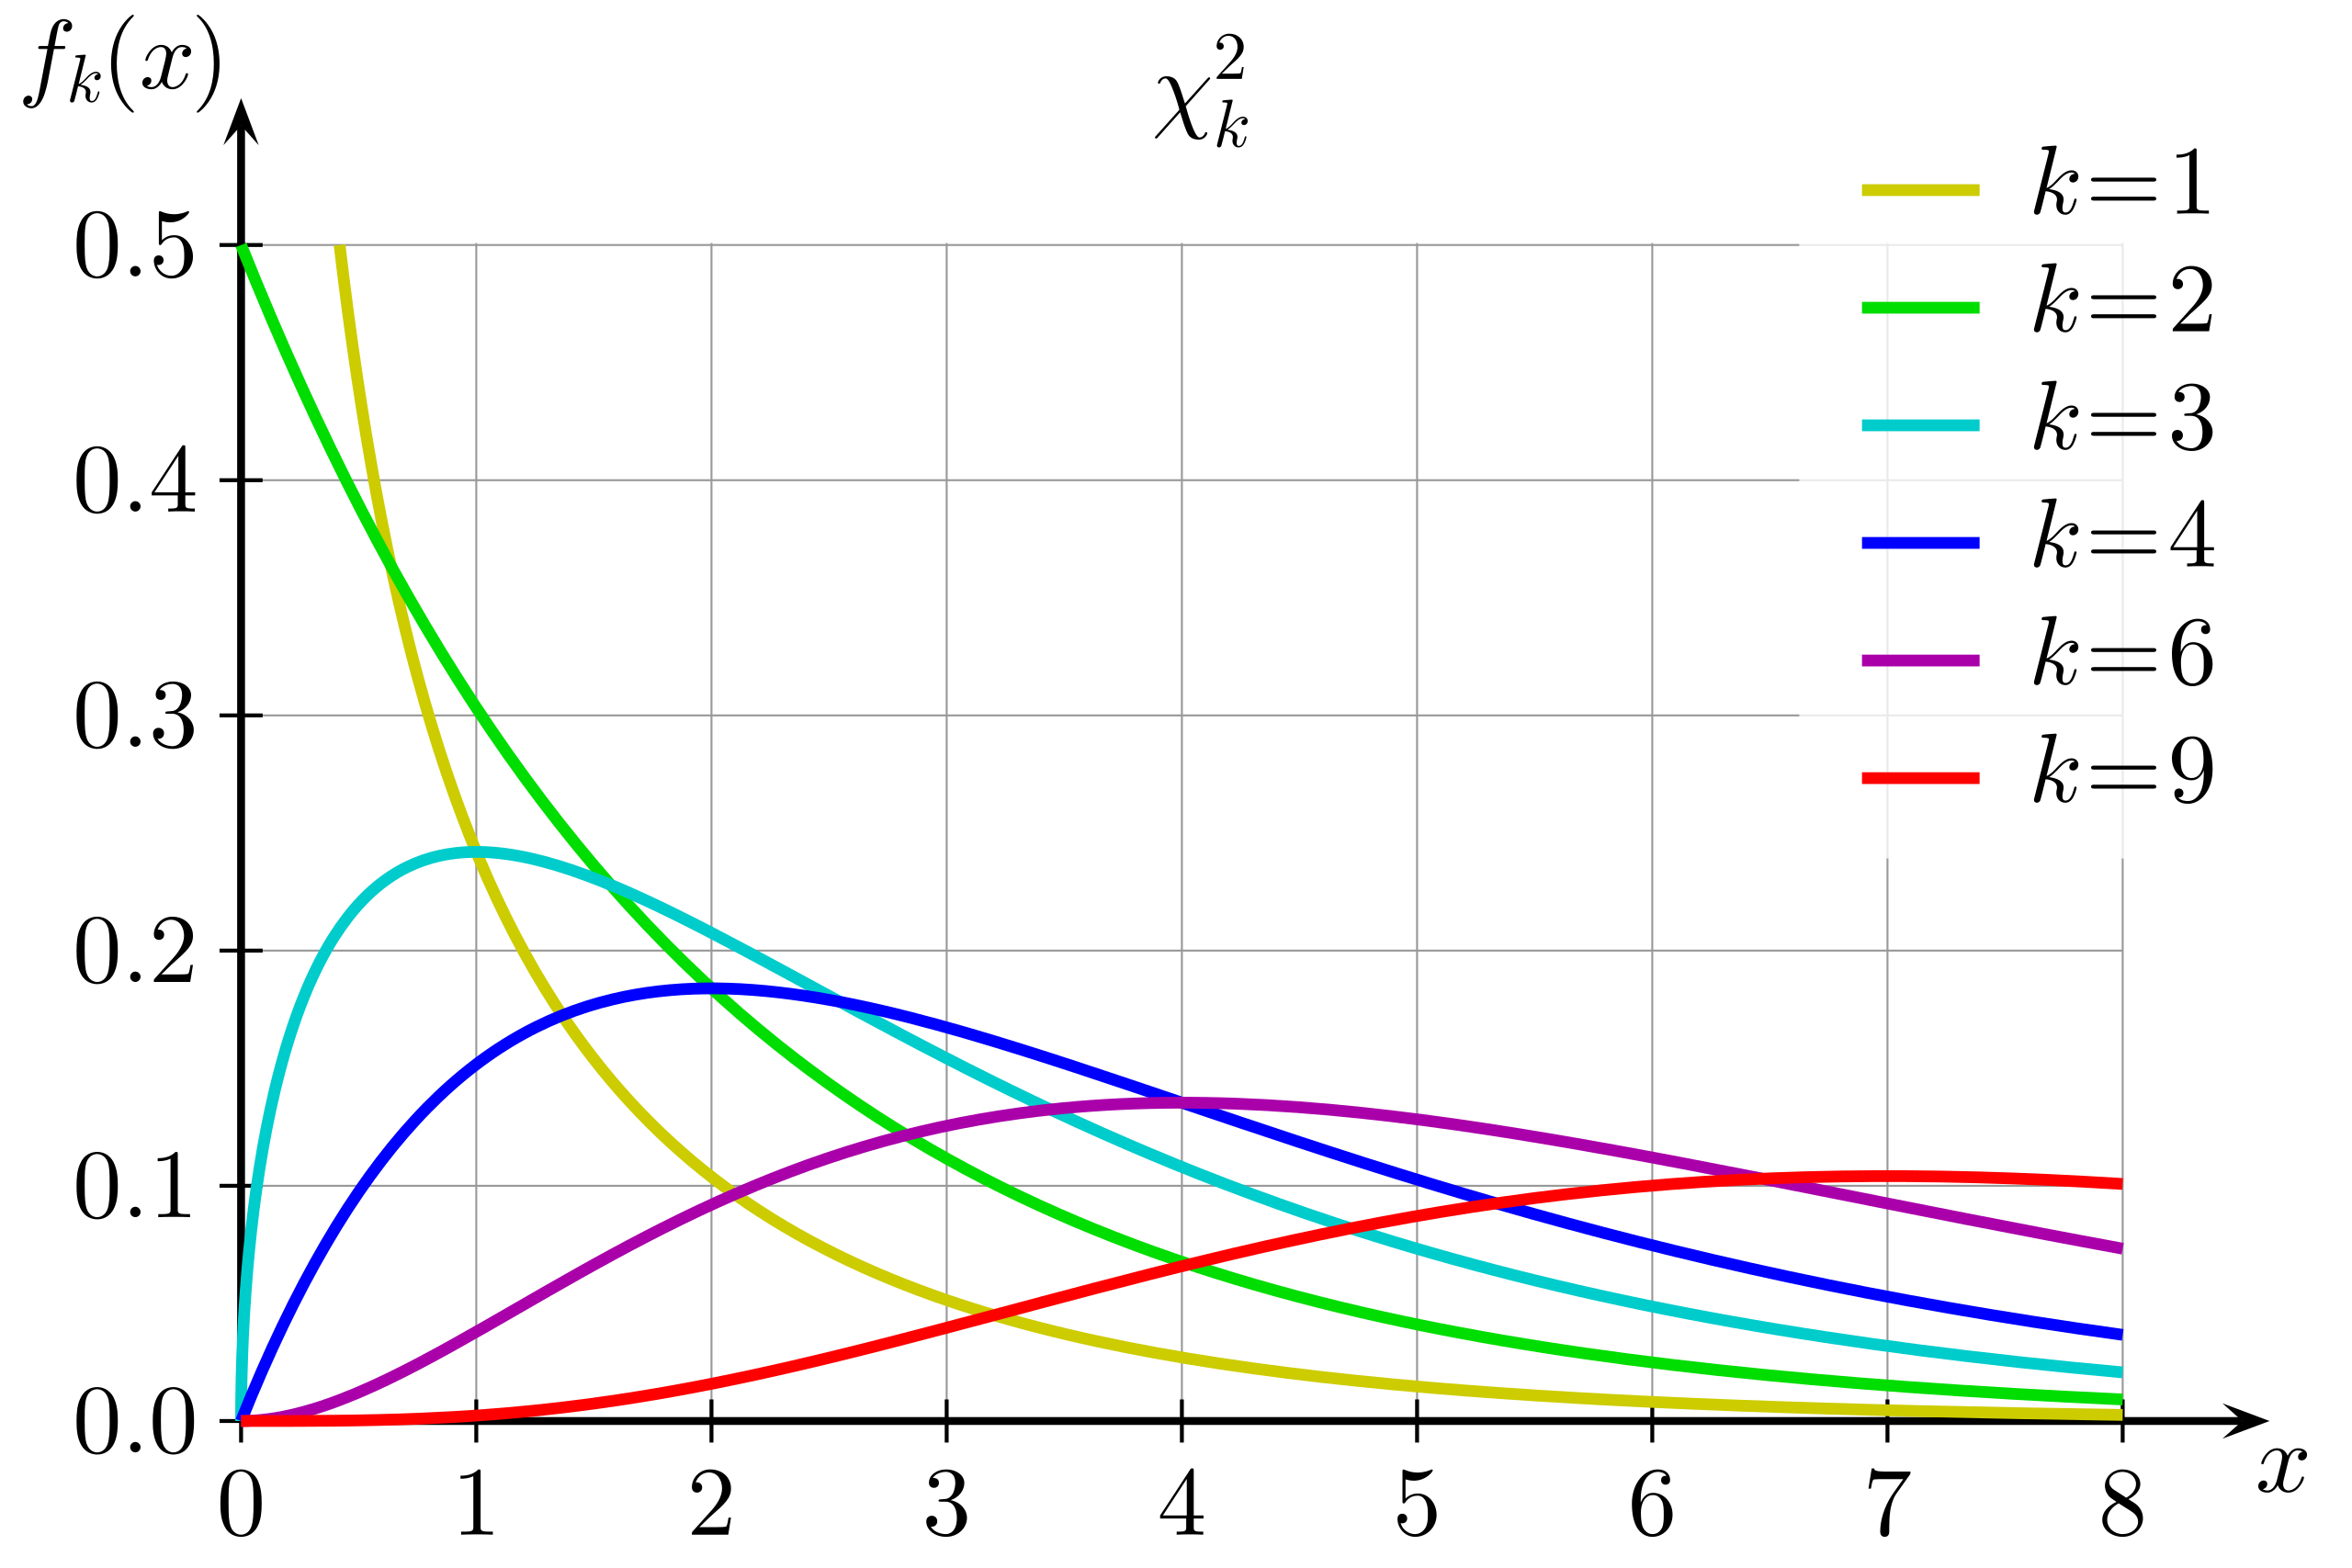
\includegraphics{Chi-square_pdf.png}
\caption{image}
\end{figure}

As shown it is a skewed dist, as v increases the skew decreases.

\hypertarget{how-do-you-test-for-bias}{%
\subsubsection{How do you test for
bias?}\label{how-do-you-test-for-bias}}

The difference between the expected (non bias result) and the observed
result will indicate bias.

Both size and relative size matter:

\((O-E) * (O-E)/E = (O-E)^2/E\)

O: Observed, E: Expected

\hypertarget{what-value-is-used-to-determine-goodness-of-fit-between-two-models}{%
\subsubsection{What value is used to determine goodness of fit between
two
models?}\label{what-value-is-used-to-determine-goodness-of-fit-between-two-models}}

\(X^2 = \sum^{m}_{i=1} (O_i - E_i)^2/E_i\)

Where m is the number of different outcomes for each model (columns).

\textbf{Large value of \(X^2\) suggest a lack of fit}

\hypertarget{how-does-x2-relate-to-chi-squared}{%
\subsubsection{\texorpdfstring{How does \(X^2\) relate to Chi squared
?}{How does X\^{}2 relate to Chi squared ?}}\label{how-does-x2-relate-to-chi-squared}}

Chi squared dist approximately shows the probability distribution of
\(X^2\), if the freq values \textgreater{} 5 :

\(X^2 = \Chi^2_{m-1}\)

\hypertarget{what-is-a-contingency-table}{%
\subsubsection{What is a contingency table
?}\label{what-is-a-contingency-table}}

A table with more than two variables being measured against (two+ rows)

The degree of freedom is : \(v= (r-1)(c-1)\)

r: rows, c: columns

\textbf{If \(X^2\) is within the chi squared 95\% interval it should be
accepted as independent}

\hypertarget{what-should-you-do-with-a-2x2-table}{%
\subsubsection{What should you do with a 2x2 table
?}\label{what-should-you-do-with-a-2x2-table}}

Can use the alternative:

\(X^2 = \sum (|O-E|-0.5)^2/E\)

\end{document}
